%\documentclass{article}
\documentclass[nofootinbib,amsmath,amssymb,10pt,eqsecnum, twocolumn]{revtex4-1}
\usepackage{graphicx, amsmath, amsmath, amssymb}
\usepackage[caption=false]{subfig}
\usepackage[breaklinks, colorlinks, citecolor=blue]{hyperref}
%\usepackage[maxbibnames=4]{biblatex}
\usepackage{color}
\usepackage{float}
\usepackage{natbib,hyperref,ifthen}
%------------ May need to comment out this -----------
%\usepackage{epstopdf}
%-----------less/greater than approx eq to--------------
\newcommand{\lta}{\mbox{\small\raisebox{-0.6ex}{$\,\stackrel
{\raisebox{-.2ex}{$\textstyle <$}}{\sim}\,$}}}
\newcommand{\gta}{\mbox{\small\raisebox{-0.6ex}{$\,\stackrel
{\raisebox{-.2ex}{$\textstyle >$}}{\sim}\,$}}}   
%-------------------------------------------------------
\newcommand{\edT}{\eta_{\Delta T}}
\newcommand{\nueff}{\nu_{\rm eff}}
\newcommand{\Tobs}{\tilde{T}_A^F}
\newcommand{\sigpix}{\sigma_{\rm pix}}
\newcommand{\sigsr}{\sigma_{\rm sr}}
\newcommand{\Tfa}{\Tobs}
\newcommand{\Tmod}{\hat{T}_A^F}
\newcommand{\Planck}{{\em Planck}}
\newcommand{\WMAP}{{\em WMAP}}
\newcommand{\un}{\, \rm}
\newcommand{\al}{\alpha}
\newcommand{\be}{\beta}
\newcommand{\ga}{\gamma}
\newcommand{\de}{\delta}
\newcommand{\s}{\sigma}
\newcommand{\pd}{\partial}
\newcommand{\brpd}{\bar{\partial}}
\newcommand{\Chr}[2]{\Gamma^{#1}{}_{\!#2}}
\newcommand{\brChr}[2]{\overline{\Gamma}^{#1}{}_{\!#2}}
\newcommand{\brg}{\bar{g}}
\newcommand{\brR}{\bar{R}}
\newcommand{\brG}{\bar{G}}
\newcommand{\brT}{\bar{T}}
\newcommand{\brLambda}{\overline\Lambda}
\newcommand{\brdel}{\overline\nabla}
\newcommand{\dd}{{\rm d}}
\newcommand{\jump}[1]{ \left[ #1 \right]^+_- }
\newcommand{\avrg}[1]{ \left\langle #1 \right\rangle^+_- } 
\newcommand{\Boxbar}{\overline{\Box}}
\newcommand{\diag}{\mbox{diag}}
\newcommand{\eps}{\varepsilon}
\newcommand{\oem}{{\cal T}}
\newcommand{\brW}{\overline{\cal W}}
\newcommand{\wave}{\square}
\newcommand{\brwave}{\overline{\square}}
\newcommand{\brkap}{{\bar\kappa}}
\newcommand{\bo}{\beta_0}
\newcommand{\binf}{\beta_{\!_\infty}}
\newcommand{\boldomega}{{\bf \omega}}
\newcommand{\appleq}{\raisebox{-3pt}{\makebox[14pt]{$\stackrel{\textstyle<}
{\sim}$}}}
\newcommand{\blockmatrix}[4]{\left( \begin{array}{c|c} #1
& #2 \\ \hline #3 & #4 \end{array} \right)}
\newcommand{\mbar}{{\bar m}}
\newcommand{\beq}{\begin{equation}}
\newcommand{\eeq}{\end{equation}}
\newcommand{\btheta}{{\bf \hat{n}}}
\newcommand{\absmax}{{$|\mbox{Max}|$}}
\renewcommand{\arraystretch}{1.6}
\newcommand{\qsubrm}[2]{{#1}_{\scriptsize{\textrm{#2}}}}
\def\ee{\end{equation}}
\def\bea{\begin{eqnarray}}
\def\eea{\end{eqnarray}}
\def\bse{\begin{subequations}}

\bibliographystyle{arxiv}

\def\mnras{MNRAS}
\def\jcap{JCAP}

\newcommand\comment[1]{\textcolor{red}{#1}}

%-------------------------------------------------------

\begin{document}

\title{Deep Recurrent Neural Networks for Supernovae Classification}

\author{Tom Charnock} \email{tom.charnock@nottingham.ac.uk}
\affiliation{School of Physics \& Astronomy\\
University of Nottingham,
Nottingham, NG7 2RD, England}

\author{Adam Moss} \email{adam.moss@nottingham.ac.uk}
\affiliation{School of Physics \& Astronomy\\
University of Nottingham,
Nottingham, NG7 2RD, England}

\date{\today}

\begin{abstract}
   We apply deep recurrent neural networks, which are capable of learning complex sequential information, to classify supernovae\footnote{Code available at \href{https://github.com/adammoss/supernovae}{https://github.com/adammoss/supernovae}}. The observational time and  filter fluxes are used as inputs to the network, but since the inputs are agnostic additional data such as host galaxy information can also be included. Using the Supernovae Photometric Classification Challenge (SPCC) data, we find that deep networks are capable of learning about light curves, however the performance of the network is highly sensitive to the amount of training data.  For a training size of 50\% of the representational SPCC dataset (around $10^4$ supernovae) we obtain a type Ia vs non type Ia classification accuracy of 94.8\%, an area under the Receiver Operating Characteristic curve AUC of 0.986 and a SPCC figure-of-merit $F_1=0.64$. We also apply a pre-trained model to obtain classification probabilities as a function of time, and show it can give early indications of supernovae type. Our method is competitive with existing algorithms and has applications for future large-scale photometric surveys. 
   \end{abstract}

\maketitle

\section{Introduction}

Future large, wide-field photometric surveys such as the Large Synoptic	Survey Telescope (LSST) will produce a vast amount of data, covering a large fraction of the sky every few nights. The amount of data produced lends itself to new analysis methods which can learn abstract representations of complex data. Deep learning is a powerful method for gaining multiple levels of abstraction, and has recently produced state-of-the-art results in tasks such as image classification and natural language processing. There are several types of deep learning architectures, such as convolutional neural networks, deep belief networks and recurrent neural networks (see~\cite{0483bd9444a348c8b59d54a190839ec9} for an excellent overview of deep learning and refs. within for more details).

There are many applications of deep learning for large photometric surveys, such as: (1) the measurement of galaxy shapes from images; (2) automated strong lens identification from multi-band images; (3) automated classification of supernovae; (4) galaxy cluster identification. In this paper we will focus on supernovae classification using deep recurrent neural networks. The LSST, for example, is expected to find over $10^7$ supernova~\cite{2009arXiv0912.0201L}. However,  it is estimated that only 5000 to 10,000\footnote{Although these numbers are not guaranteed.} will be spectroscopically confirmed  by follow up surveys~\cite{2013arXiv1311.2496M}, so classification methods need to be developed  for photometry.  All previous approaches to automated classification~\cite{Newling:2010bp, Karpenka:2012pm, Lochner:2016hbn} have first extracted features from supernovae light curves before using machine learning algorithms.  One of the advantages of deep learning is replacing this feature extraction. 

In this work we will use {\em supervised} deep learning. During training, the machine is given inputs and produces a set of output predictions.  It is also given the correct set of outputs. An objective loss function then measures the error between the predicted and target outputs, and the machine updates its adjustable parameters to reduce the error. It can then make predictions for unknown outputs.

\begin{figure}
\centering
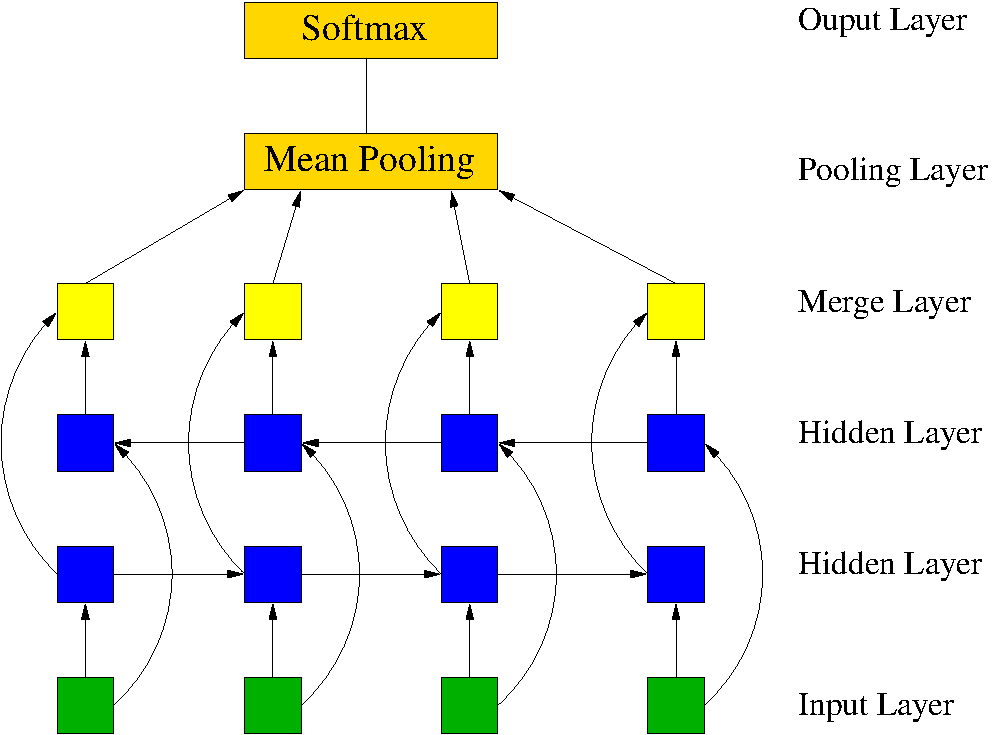
\includegraphics[width=88mm, angle=0]{1.pdf}
\caption{\label{fig:network} Bidirectional recurrent neural network for sequence classification. The input vectors at each sequential step are fed into a pair of bidirectional hidden layers, which can propagate information forwards and backwards. These are then merged to obtain a consensus view of the network, and finally a softmax layer computes classification probabilities. 
 }
\end{figure}

{\em Recurrent neural networks} (RNNs) are a class of artificial neural network  that can learn about sequential data. They are commonly used for tasks such speech recognition and language translation, but have several possible applications in astronomy  and cosmology for processing temporal or spatial sequential data. RNNs have several properties which makes them suitable for sequential information. The inputs to the network are flexible, and they are able to recognise patterns with noisy data (for example the context of a word in a sentence relative to others can vary, or a time stream can contain instrument noise). 

The main problem with vanilla RNNs  is that they are unable to store long-term information, so inputs at the end of a sequence have no knowledge of inputs at the start. This is a problem if the data has long-term correlations. Several types of RNNs have been proposed to solve this problem, including {\em Long Short-Term Memory} (LSTM)~\cite{LSTM} and {\em Gated Recurrent Unit} (GRU)~\cite{2014arXiv1412.3555C} units. These are similar in concept, in that information is able to flow through the network via a gating mechanism. One further problem with RNNs is that information is only able to flow in one direction. In {\em bidirectional} RNNs information is able to pass both forwards and backwards. Bidirectional LSTM networks have been shown to be particularly powerful for supervised sequence labelling, where sequential data is accompanied by a set of discrete labels. 

The architecture of a typical bidirectional RNN for sequence labelling is shown in Fig.~\ref{fig:network}, where the squares represent {\rm neurons}. In this case the inputs, which are vectors at each sequential step, are connected to two hidden RNN layers, which can be either vanilla RNN or memory units.  Each hidden layer contains a number of hidden units (capable of storing information), and in each layer information flows either forwards or backwards,  but no information passes between the two directions. Several hidden layers can be stacked to form {\em deep} neural networks. Deep networks are capable of learning higher-level temporal or spatial representations, and complex relationships between the inputs and outputs.

The output from the final set of hidden layers in each direction is merged at each sequential step, and mean pooled (averaged) over all steps to obtain a consensus view of the network\footnote{We find that obtaining a consensus view improves the performance of the network.}. Finally, the mean output is fed to a {\em softmax} layer, which takes an input vector ${\bf z}$ and returns normalised, exponentiated outputs for each class label $i$, $\exp(z_i) / \sum_{i} \exp(z_i)$, i.e. a vector of probabilities.

 In the network, each neuron is connected to another by a weight matrix, and the optimal weights are found by back-propagating the errors from a {\em loss function} of the output layer. For classification problems, this is typically the categorical cross-entropy between predictions and targets, defined as 
\begin{equation}
L= -\sum_{i,j} t_{i,j} \log \left( p_{i,j} \right)
\end{equation}
where $i,j$ run over the class labels, $t_{i,j}$ are the targets for each class (either 0 or 1) and $p_{i,j}$ are the predicted probabilities. Back-propogation essentially takes the derivative of the loss with respect to the weights $W$ of the output layer, $\partial L/\partial W$, and uses the chain rule to update the weights in the network.

\section{Example Data}

In this paper we will consider data from the Supernovae Photometric Classification Challenge (SPCC)~\cite{Kessler:2010wk,Kessler:2010qj}, which consists of a set of 21319 simulated supernove light curves.  Each supernovae sample consists of a time series of flux measurements, with errors, in the $g, r, i, z$ bands (one band for each timestep), along with the position on the sky and dust extinction. An example set of light curves is shown in Fig.~\ref{fig:lightcurve}. 

Due to the format of the input data, we first do a small amount of data processing to obtain values of the $g, r, i, z$ fluxes and errors at each sequential step.  First, we assume the time sequence begins at day 0 for each supernovae, rather than counting days forwards and backwards from the maxima of the light curve. Next, for observations less than $\sim1$ hour apart, we group the $g, r, i, z$ values into a single vector, ensuring there is at most one filter type in each group. If there is more than one filter type, we further subdivide the group using a finer time interval.  We take the time of the group to be the mean time of its individual observations, which is reasonable as the time intervals are small compared to the characteristic time of the light curve. 

 Observations are then of the form in Tab.~\ref{tab:augment}, where any missing values are denoted by a dash. In order to impute the missing value of $i$, we use {\em data augmentation} and randomly select a value between $i_1$ or $i_3$. We make 5 random augmentations of all missing data, thereby increasing the size of the dataset by a factor of 5. We can test the importance of this by training each augmentation separately and  comparing the change in accuracy, which we find is $\sim 1\%$. Training with multiple augmentations at once gives the best performance, since the network will learn  to ignore random filled values. 

\begin{table}[htdp]
\begin{center}
\begin{tabular}{|c|c|c|c|c|} \hline  
 Time & g & r & i & z \\ \hline \hline 
$ t_1$  & $g_1$ & $r_1$ &$ i_1$ & $z_1$ \\ \hline 
$ t_2$  & $g_2$ & $r_2$ &$  - $ & $z_2$ \\ \hline 
$ t_3$  & $g_3$ & $r_3$ &$ i_3$ & $z_3$ \\ \hline 
 \end{tabular}
\end{center}
\label{tab:augment}
\caption{Data augmentation of missing observations. The missing data is replaced randomly by a value between $i_1$ or $i_3$.}
\end{table}%

\begin{figure}
\centering
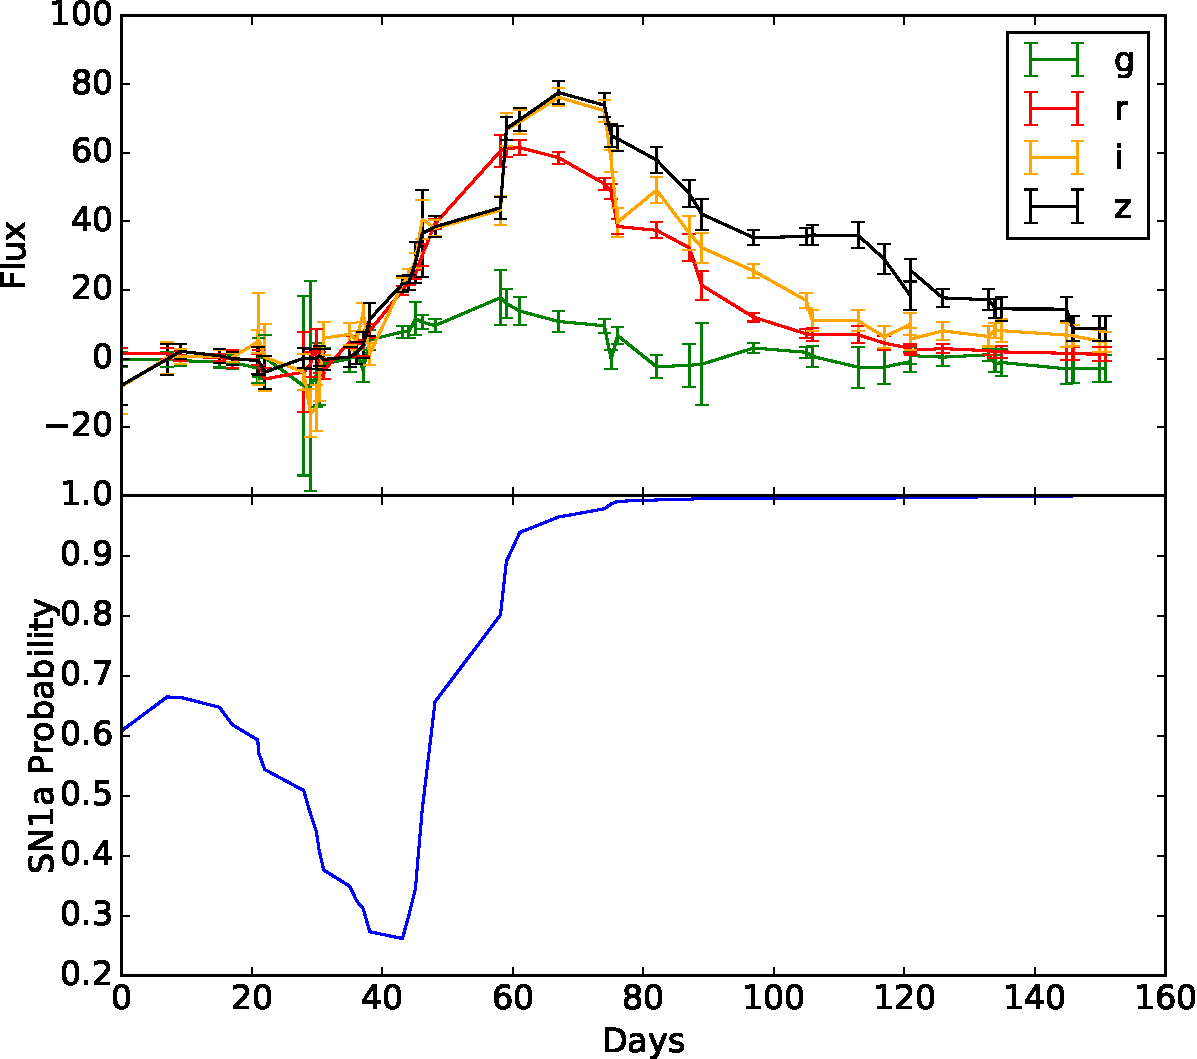
\includegraphics[width=88mm, angle=0]{2.pdf}
\caption{\label{fig:lightcurve} (Top) Example light curve in the 4 $g, r, i, z$ bands for SN ID 551675 (a type Ia) in the Supernovae Photometric Classification Challenge data~\cite{Kessler:2010wk}. The data has been processed using augmentation so there is a $g, r, i, z$ value at each sequential step. (Bottom) Type Ia probability as a function of time from a 2 layer LSTM model, trained with around $10^4$ supernovae and SN 551675 excluded. The final probability gives $99.5\%$ confidence that the supernovae is of type Ia. 
 }
\end{figure}


The data comes in two types, those with and those without the  host galaxy photometric redshift. Each dataset is split into a training and test set, with the training set containing a spectroscopically confirmed supernovae type and redshift. It is important that augmented data with the same supernovae ID go into either the training {\em or} test set, not a mix of both, otherwise the training and test data will not be independent. The original SPCC data consisted of 1103 training samples. The answer keys were subsequently made available for the test set~\cite{Kessler:2010qj}. 

The input vector to each sequential step then consists of: the time in days since the first observation; the flux in each of the 4 bands; the flux errors in each of the 4 bands; the RA and Dec; the dust extinction; and the host photo-z if relevant. Whilst we do not expect some of these variables to impact the classifier accuracy, we do not attempt any feature engineering and leave it to the network to decide if they are relevant. 

RNNs typically perform better with more training data, so for training purposes we use the SPCC test set with answer keys (which is a non-biased representational dataset\footnote{The original SPCC training set was non-representational.}), and select a random fraction to act as the training set. We consider 1103 supernovae (a training fraction of 0.052), the same size as the original challenge, and fractions of 0.25 and 0.5 (around 5000 and $10^4$ supernovae respectively), nearly an order of magnitude larger, and closer to the number likely to be followed up for the LSST. The training performance of RNNs is also improved if the data is processed in mini-batches. In order to do this the input data must be of the same length, so we set the sequence length to be the maximum length over all supernovae observations, and prepend the input with padding. In training the network we ensure the padding is ignored by masking the padded input. 

The goal of the classifier is to determine the supernovae type in the test set. We consider two problems, the first being to categorise two classes (type Ia vs non type Ia), and the second to categorise three classes (supernovae types 1, 2 and 3). We denote these as  `SN1a' and  `123' respectively.  

We use several metrics to assess the classifier. The simplest is the accuracy, defined as the ratio between the number of correct predictions and total number of predictions. With two classes, a random classifier would have an accuracy of 0.5, and with three classes, an accuracy of 1/3.

Next are a variety of metrics coming from the {\em confusion matrix} of predictions.  For binary classification problems, the confusion matrix splits predictions into true positives (TP), false positives (FP),  false negatives (FN), and true negatives (TN). We consider the purity (also known as precision) and completeness (also known as recall) of the classifier. These are defined as 
\begin{equation}
{\rm Purity} = \frac{{\rm TP}}{{\rm TP}+{\rm FP}}\,, \quad {\rm Completeness} = \frac{{\rm TP}}{{\rm TP}+{\rm FN}}\,.
\end{equation}
We evaluate these for each class separately vs `the rest' (e.g. type Ia vs non type Ia). The SPCC also defined the $F_1$ figure-of-merit for the SN1a classification problem. This is 
\begin{equation}
F_1 = \frac{1}{{\rm TP}+{\rm FN}} \frac{{\rm TP}^2}{{\rm TP}+3 \times {\rm FP}}\,,
\end{equation}
so false positives (incorrectly classifying a non type Ia supernovae as a type Ia) are penalised more heavily.

Finally, we also calculate  the Area Under the Curve (AUC). The AUC is the area under the curve of the TP rate vs FP rate, as the threshold probability for classification is increased from 0 to 1. A perfect classifier has an AUC of 1, and a random classifier 0.5. For multi-class problems, we calculate the AUC for each class vs the rest, and take an unweighted average to give the final AUC score. 

\section{Network Architecture}

We consider several combinations of the network architecture. For the RNN type in the hidden layers, we test both vanilla RNN and long-term memory (LSTM and GRU) units. We also consider unidirectional  and bidirectional networks. For the unidirectional network, we fix the direction to be forwards. For the bidirectional network, we fix the number of hidden units in each RNN layer to be equal for the forward and backward directions. 

We also test stacking two sets of layers to form a deep network.  In the unidirectional case we stack two hidden layers. In the bidirectional case the two stacks consists  of a pair  of forwards and backwards layers.  We denote the number of hidden units in a network with a  single stack by $[h_1]$, and the number of hidden layers in a two stack model by $[h_1, h_2]$. We vary the number of hidden units, testing h=[4], [8], [16], [32], [4,4], [8,8], [16,16] and [32,32]. We do not go beyond a stack of two layers due to the limited size of the dataset. 

For each network we perform 5 randomised runs over the training data to obtain the classifier metrics. We define the loss function as the categorical cross-entropy between the predictions and test data. The network weights were trained using back-propogation with the `Adam' updater~\cite{2014arXiv1412.6980K}. Mini-batches of size 10\footnote{If training with a GPU larger mini-batches are recommended to make use of the GPU cores.} were used throughout, and each model was trained over approximately 200 {\em epochs}, where each epoch is a full pass over the training data.

\section{Results}

\begin{figure}
\centering
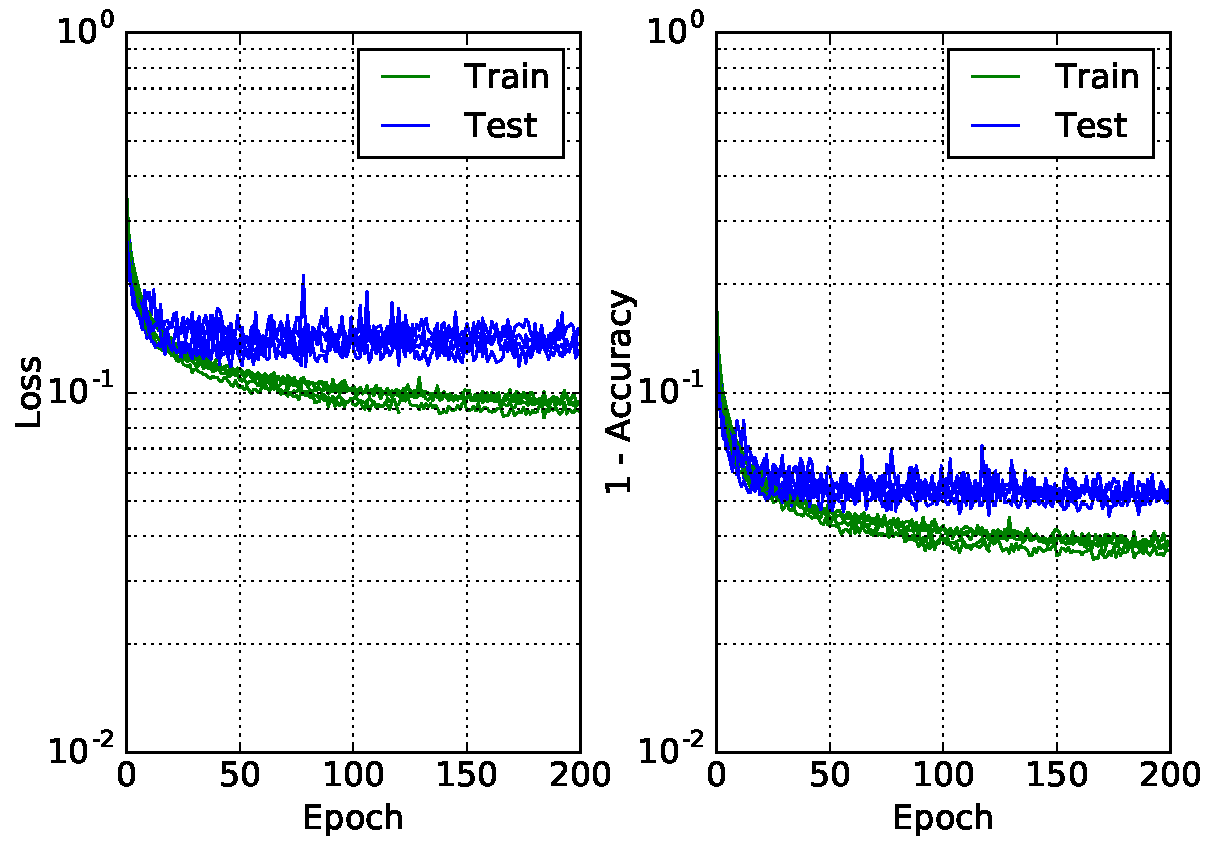
\includegraphics[width=88mm, angle=0]{3.pdf}
\caption{\label{fig:loss} (Left) Training loss (green) vs test loss (blue) for a unidirectional 2 layer  LSTM network with 16 hidden units in each layer. (Right) Training accuracy (green) vs test accuracy (blue) for the same network.  }
\end{figure}

A dataset of 21319 is relatively small by deep learning standards. Furthermore, the `feature space' of supernovae light curves is significantly smaller than, say using RNNs to learn about language. We therefore need to be careful about {\em over-fitting}. Over-fitting arises when the network fits noise between the inputs and outputs of the training data, which do not exist in the test data. It can typically be detected by comparing the loss of the training and test data. If the loss of training data continues to decrease, but the loss of the test data increases, this is a sure sign of over-fitting. On the other hand, if no sign of over-fitting is observed, the network is not usually complex enough to fully learn the relationship between inputs and outputs (called {\em under-fitting}).  

For a training fraction of 0.5, we found the best architecture was a deep 2 layer network with unidirectional LSTM units. Bidirectional units did not significantly improve the test accuracy and made the network more difficult to train. There was a marked improvement in test accuracy using 16 hidden units in each layer rather than 8, but too much over-fitting occured using 32 hidden units. Over-fitting was still an issue for 16 hidden units,  but we make use of a technique called {\em dropout}~\cite{JMLR:v15:srivastava14a} to regularize this. Dropout  sets a random fraction of connections to 0 at each update during training {\em only}, which prevents the units from adapting too much. We apply dropout only to non-recurrent connections after each hidden layer. 

In Fig.~\ref{fig:loss} we show the training and tests losses for such a network, with a dropout of $0.5$, applied to type Ia vs non type Ia classification with host galaxy photo-z information. Without dropout the training loss would continue to fall and the test loss would rise. For 5 randomised runs, after training for  200 epochs, we obtain a classification accuracy of $94.8 \pm 0.2$\%, an AUC of $0.986 \pm 0.001$ and $F_1 = 0.64 \pm 0.01$. The corresponding type Ia purity and completeness are 87\% and 92\% respectively. A summary of results for this network can be found in Tabs.~\ref{tab:05_SN1a} and~\ref{tab:05_123}. It can be seen that the inclusion of host galaxy photo-z does not significantly improve the classifier performance.  

\begin{table}[t!]
\begin{tabular}{|c | c | c | c | c |} \hline 
AUC & Accuracy & F1 & Host z \\ \hline 
$ 0.986 \pm  0.001$ &  $  94.8 \pm 0.2\% $ & $  0.64 \pm 0.01  $ & T  \\
$ 0.981 \pm  0.002$ &  $  93.6 \pm 0.3\% $ & $  0.60 \pm 0.02  $ & F  \\ \hline
\end{tabular}
\caption{\label{tab:05_SN1a} Summary of results for  type Ia vs non type Ia classification with a training fraction of 0.5. The network used is a 2 layer LSTM, each with 16 hidden units, and a dropout of 0.5.}
\end{table}

\begin{table}[t!]
\begin{tabular}{|c | c | c | c | c |} \hline 
AUC & Accuracy & Host z  \\ \hline 
$ 0.971  \pm 0.003 $ &  $  90.4  \pm 0.4 \% $ & T  \\
$ 0.958 \pm  0.007 $ &  $   88.8 \pm 1.0 \% $ & F \\ \hline
\end{tabular}
\caption{\label{tab:05_123} Summary of results for three class categorisation (supernovae types 1, 2 and 3). The model is the same as in Tab.~\ref{tab:05_SN1a}}
\end{table}

One advantage of our approach is that light curve data can be directly inputted to a {\em pre-trained} model to give very fast evaluation ($<1\,$s) of supernovae type. In the lower panel of Fig.~\ref{fig:lightcurve} we input the light curve, as a function of time, of a type Ia supernovae (excluded from training) to the pre-trained 2 layer LSTM model discussed above. The classifier (type Ia vs non type Ia) is initially unsure of classification, with a type Ia probability of around 0.5. The probability then decreases slightly, but rapidly increases near the peak of the light curve. The classifier has high confidence the supernovae is of type Ia at around 60 days, and the final probability is excess of $99.5\%$.  This method could therefore be useful to give early indication of supernovae type in  surveys.

We also test the same model using a training fraction of 0.25 (around 5000 supernovae), closer to the lower  end of the number likely to be followed up for the LSST. Again, after 5 randomised runs and training for 200 epochs we obtain an accuracy of $93.3 \pm 0.4\%$, an AUC of $0.978 \pm 0.002$ and $F_1 = 0.57 \pm 0.02$. The corresponding type Ia purity and completeness are 85\% and 87\% respectively. The $F_1$ metric, for example, has degraded by $\sim10\%$ for a reduction in data of $50\%$.

For $5.2\%$ of the representative SPCC data, the training dataset is so small that over-fitting is more severe. Using the same 2 layer LSTM network with 16 hidden units and a dropout of 0.5 we find a notable increase in the test loss after $\sim 20$ epochs, but the accuracy and other metrics remain relatively constant ($F_1$ values, for example, of 0.35 to 0.4 were obtained). The reason for this apparent discrepancy is that the accuracy, say, simply takes the maximum value of the softmax output layer. For example, a 2 class problem with output probabilities [0.6, 0.4] and target [1, 0] has the same accuracy as one with output probabilities [0.8, 0.2]. The loss in the latter case would be lower however, and represents increased confidence of the network in its predictions. We therefore reject models with severe over-fitting and an increasing cross-entropy loss, at the expense of metrics such as $F_1$, and decrease the model complexity. 

For a training fraction of  $5.2\%$ we find a single layer LSTM network, with 4 hidden units, and a dropout of 0.5 satisfies this criteria. For 5 randomised runs, after training for  200 epochs, we obtain a classification accuracy of $85.9 \pm 1.2$\%, an AUC of $0.910 \pm 0.012$ and $F_1 = 0.31 \pm 0.03$. The corresponding type Ia purity and completeness are 72\% and 66\% respectively.

\section{Conclusions}

We have presented a new method for performing  photometric classification of supernovae. Machine learning methodology has previously been applied to SPCC classification~\cite{Newling:2010bp, Karpenka:2012pm, Lochner:2016hbn}. These all employ a two step process, where features are first extracted by some method before classification. In our approach light curves are used directly as inputs to a recurrent neural network, which is able to learn information from the sequence of observations.

Using post SPCC data, we obtain results which are competitive with previous approaches.  Although we have trained the network on the cross-entropy loss  and not the $F_1$ score, for the same sized dataset of $\sim10^3 (10^4)$ supernovae (including host galaxy photo-z), \cite{Karpenka:2012pm} obtained $F_1$ values of 0.33 (0.58), and \cite{Newling:2010bp} values of 0.42 (0.57), compared to our  0.31 (0.65). Recurrent neural networks  therefore compare very well with a larger training  set. The performance isn't  quite as good with a smaller training set, possibly due to the network having to learn from no prior information about (noisy) light curves. This is also seen in~\cite{Lochner:2016hbn}, which obtains improved metrics for only a small training fraction with a combination of feature extraction and machine learning. As well as finding competitive results for the final metrics, we have shown that it is possible to give fast, early evaluation of supernovae type using pre-trained models. This is possible since the light curve can be fed to the model directly without needing any feature extraction.  

There are several possibilities for future work. One of the advantages of recurrent neural networks is that inputs are agnostic, so the impact of any additional inputs could be explored. It would be possible, for example, to even pass the raw images in each filter though a convolutional network and use those as inputs. We have considered a representative training sample, but spectroscopic follow up surveys may be biased. The performance of the network could be measured against selection bias, and the results used to inform the best follow up strategy.  Further work could also be performed to optimise the early detection probability of the network.  Finally, to improve performance in the small data regime one can use {\em transfer learning.} Here, a more complex network is pre-trained on simulations or existing data from other surveys, then the weights of the network are fine-tuned on the new, smaller dataset. The simulated SPCC data used in this work are based on the DES instrument, so it would be interesting to apply transfer learning to real DES data. 

\section*{Acknowledgements}

We appreciate helpful conversations with Steven Bamford, Simon Dye, Mark Sullivan and Michael Wood-Vasey, and Natasha Karpenka, Richard Kessler and Michelle Lochner for help with data acquisition. T. C. is supported by a STFC studentship, and A. M. is supported by a Royal Society University Research Fellowship.

\bibliography{bib}

\end{document}
